\begin{section}{Fisher Information Content}
  \label{sec:fisherinfo}
  Mathamatically, the Fisher information $I$ of the initial scale
  invariant matter power spectrum, $A$, is defined as
  \begin{align}
    I_A \equiv -\left\langle \frac{\partial ^2 \mathrm{ln \Largr}}{\partial  \mathrm{ln} A ^2}\right\rangle,
    \label{eq:fisherdefine}
  \end{align}
  where $\Largr$ is the likelihood \cite{bib:Tegmark1997}.  
  In this paper, the word \enquote{information} and the symbol \enquote{$I$} both implicitly 
  mean cumulative Fisher information 
  of $A$. For Gaussian
  fields, the likelihood depends on parameters only through
  power spectrum $P(k)$, so $I$ can be written as 
  \begin{align}
    I = - \left\langle \sum_{k,k'} \frac{\partial \mathrm{ln} P(k)}{\partial \mathrm{ln} A} 
    \frac{\partial ^2 \mathrm{ln \Largr}}{\partial \mathrm{ln} P(k) \partial \mathrm{ln} P(k')}
    \frac{\partial \mathrm{ln} P(k')}{\partial \mathrm{ln} A}\right\rangle,
    \label{eq:fisherdef2}
  \end{align}
  where the angle bracket averages over realizations
  \cite{bib:Rimes2006}.
  Eq.~\ref{eq:fisherdef2} can be written in a simpler
  form by two steps.   
  
  First, we simplify the derivative term
  $\partial \mathrm{ln} P(k)/\partial\mathrm{ln} A$.  For a given density field $\delta_a$, we can
  %conveniently decompose it into a linear and a nonlinear component
  conveniently decompose it into a correlated, linear component,
  and a uncorrelated, noise component
  \begin{align}
    \delta_a(k) = b (k) \delta _L (k) + \delta_{n}(k),
    \label{eq:decompose}
  \end{align}
  where $\delta_L$ is the linear density field, $b(k)$ is the
  bias and $\delta_{n}(k)$ is defined such that the correlation
  $\langle \delta_L(k)\delta_{n}(k) \rangle=0$.  If we correlate
  $\delta_a$ and $\delta_L$,
  \begin{align}
    \langle \delta_a(k)\delta_L(k) \rangle = b(k) \langle \delta_L(k)\delta_L(k) \rangle,
    \label{eq:correlating}
  \end{align} 
  we can solve for $b$ as
  \begin{align}
    b (k) = \frac{P _{aL}(k)}{P_{LL}(k)}.
    \label{eq:bofk}
  \end{align}
  %To find the nonlinear term, we correlate $\delta_a$ with itself,
  To find the nonlinear term, we square both sides of Eq.~\ref{eq:decompose}
  and the cross term of the right hand side vanishes,
  \begin{align}
    \langle \delta_a(k) \delta_a(k) \rangle = 
    b^2(k) \langle \delta_L(k) \delta_L(k) \rangle + \langle \delta_{n}(k)\delta_{n}(k) \rangle,
  \end{align}
  and find
  \begin{align}
    P_{aa}(k) = b^2(k) P_{LL}(k) + P_{nn}(k).
    \label{eq:powerdecompose}
  \end{align}
  With the help of Eq.~\ref{eq:bofk} and Eq.~\ref{eq:powerdecompose},
  we get
  \begin{align}
    \frac{\partial \mathrm{ln} P(k) }{ \partial \mathrm{ln} A}=
    \frac{P_{LL}(k)}{P_{aa}(k)}b^2(k)=r^2_{aL}(k).
  \end{align}

  Second, we simplify
  $\partial ^2 \mathrm{ln \Largr}/\partial \mathrm{ln} P(k) \partial
  \mathrm{ln} P(k')$
  by using the fact that its expectation value is the Fisher
  matrix.  For Gaussian fields, this is equal to the inverse of the
  covariance matrix which is diagonal with elements given by the
  number of modes in each bin (when considering $\bs{k}$ and $-\bs{k}$ as the same mode).  
  We can extend this definition to
  non-Gaussian fields, by taking into account that the covariance
  matrix is no longer diagonal \tcr{and invert it appropriately \cite{bib:Rimes2006}}.  Thus, we
  write the Fisher information in terms of matrix multiplication:
  \begin{align}
    I \left( < k_n\right) = r^2(k)^{\mathrm{T}} \left[ \mathrm{C^{-1}_{norm}} 
    ( k,k' )\right]_{<k_n} r^2(k') ,
    \label{eq:fisherformulaused}
  \end{align}
  where
  \begin{align}
    \mathrm{C_{norm}} \left( k,k' \right)=\frac{\mathrm{Cov}(k,k')}
    {\langle P(k)\rangle\langle P(k')\rangle}
  \end{align}
  is the normalized covariance matrix, and
  $r$ is the mean cross correlation of a given density field with
  $\delta_L$ and the subscript $<k_n$ indicates the matrix is set to
  zero for modes $k,k'>k_n$.  The elements of the covariance matrix are defined as
  \begin{align}
    \mathrm{Cov}\left(k,k'\right)\equiv \frac{\sum_{i,j=1}^{N}\left[ P_i \left( k \right) - 
    \langle P \left( k \right) \rangle \right]\left[ P_j \left( k' \right) - 
    \langle P \left( k' \right)\rangle \right]}{N-1},
  \end{align}
  where $N$ is the total number of simulations and angle bracket average these simulations.  

  The cross-correlation coefficient matrix, or for short the correlation matrix, 
  is defined as 
  \begin{align}
    \mathrm{Corr}\left(k,k'\right)=\frac{\mathrm{Cov}\left(k,k'\right)}
    {\sqrt{\mathrm{Cov}\left(k,k\right)\mathrm{Cov}\left(k',k'\right)}},
  \end{align}
  representing the correlation between different $k$ modes.  The
  correlation matrices for nonlinear and reconstructed power spectra
  are shown in the upper-left and lower-right sections of Fig.~\ref{fig:corrall}.
  By definition, the correlation matrix is symmetric with unit
  diagonal allowing us to overlay the two matrices.  For the
  nonlinear case, it is almost diagonal in the linear
  regime, $k \lesssim 0.07$ $h$/Mpc.  The off-diagonal
  elements are produced by strong mode coupling on nonlinear scales
  and the super-survey tidal effect which is small on linear scales
  but dominates in the weakly nonlinear regime
  \cite{bib:Kazuyuki2016}.  The correlation matrix for the non-linear
  power spectra has negative elements
  ($\mathrm{Corr} \gtrsim -0.18$), which should vanish with more
  simulations \cite{bib:Takahashi2009}.  For the reconstructed
  correlation matrix, the linear regime extend up to $k \simeq 0.3$
  $h$/Mpc.  However, the intensity of negative off-diagonal effect
  also increases ($\mathrm{Corr} \gtrsim -0.48$).

  \begin{figure}
    \centering
    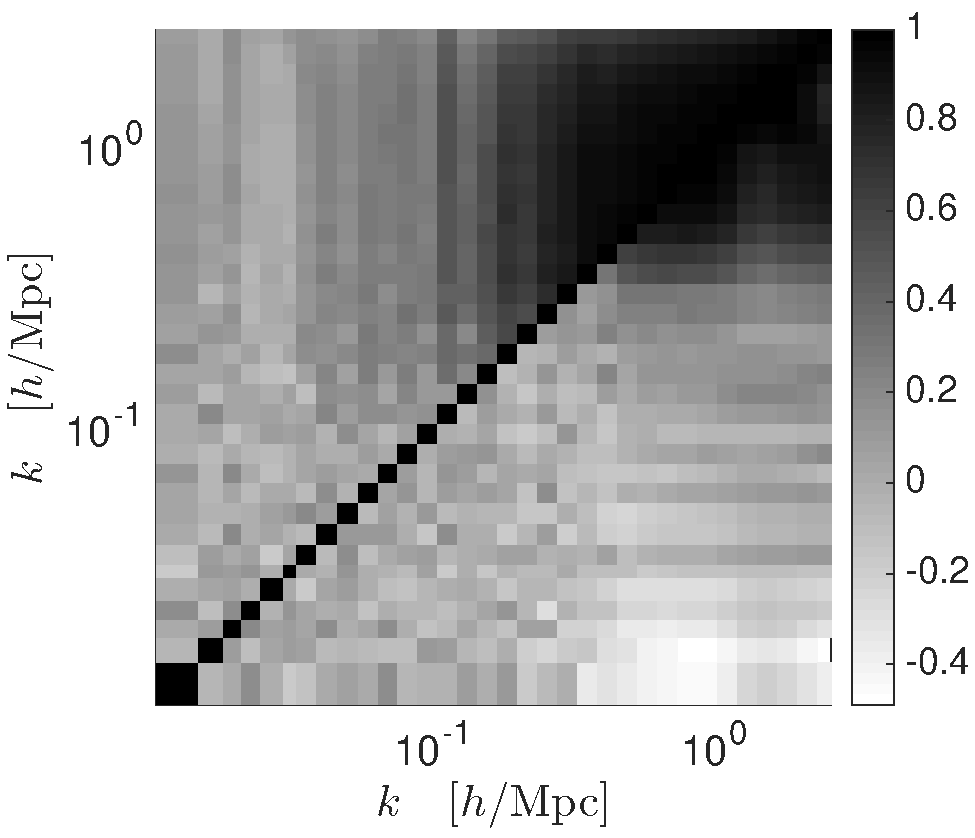
\includegraphics[width=0.48\textwidth]{fig3.pdf}
    \caption{The correlation matrix from 130 non-linear power
      spectra (the upper-left elements) and reconstructed power
      spectra (the lower-right off-diagonal elements).}
    \label{fig:corrall}
  \end{figure}

  The Fisher information is proportional to the volume. 
  We plot the Fisher information per unit volume of the power spectra of
  $\delta_S$, $\delta_L$ and $\delta_R$ in the left panel of 
  Fig.~\ref{fig:fisherinfo}. The Fisher information of the linear 
  power spectra is equal to the number of $k$ modes within the shell in 
  Fourier space, $N_k$. As expected, Fisher information of the
  $\delta_S$ drops from $\delta_L$ on scale
  $k \simeq 0.05$ $h$/Mpc, and has a flat plateau in the nonlinear
  regime, with a saturated value of
  $I \simeq 2.5 \times 10^{-5}/({\rm Mpc}/h)^3$, indicating
  the absence of independent information in the nonlinear
  regime.  In comparison, the information curve of $\delta_R$ power
  spectra keeps increasing roughly the same as the linear information
  until $k\simeq 0.3$ $h$/Mpc, and reaches a value of 
  $I \simeq 1.3 \times 10^{-3}/({\rm Mpc}/h)^3$ at $k \simeq 2.7$ $h$/Mpc,
  increased by a factor of 50.
  We compare the Fisher information given by the MM reconstruction method
  with the logarithmic density mapping method \cite{bib:Mark2009}.
  
  %This means that the MM reconstructed method can
  %strongly recover the lost information within these scales.  
  %We find that MM
  %reconstruction gives over 10 times more information than it.  
  To test the upper limit of information that the MM reconstruction can recover, 
  we calculate the Fisher information given by $\delta_E$ \cite{bib:Yu2016} indicating
  a factor of 150 boost of information on 
  $k \simeq 2.7$ h/Mpc.
  %It indicates that the MM reconstruction can give 3 times more 
  %information than our case at most. 

  In some previous works, the cross correlation $r^2$ terms are set
  to unity in Eq.~\ref{eq:fisherformulaused}, which artificially
  increases the information. To compare with their result, we plot this case in the right panel of 
  Fig.~\ref{fig:fisherinfo}.  We see that, in this case, the information of the logarithmic density
  mapping is much higher than it is in the left panel.
  In the analysis of BAO or extracting other primordial cosmological
  parameters, we should taking into account the correlation term $r^2$
  to propagate final fields back to initial conditions \citep{bib:HarnoisD2013}.
  This also answers the question of section 4
  ({\it Information about what?}) of \citet{bib:HarnoisD2013}.

  Another way to quantify the nonlinear scale is via the plateau's linear equivalent scale,
  \begin{equation}
      I_{\delta_L}(k_{\rm NL})=I_{\delta}(k\rightarrow\infty)
  \end{equation}
  i.e.,
  the scale on which linear information approaches the limit of nonlinear information
  (where the horizontal dashed line crosses $I_{\delta_{L}}$).
  Practically, we take $I_{\delta}(k\rightarrow\infty)$ to be
  $I(k=2.7$ $h$/Mpc) where $k$ is large enough.  We find that
  for $\delta_S$, $k_{\rm NL}\simeq 0.15$ $h$/Mpc.
  The MM reconstruction increases $k_{\rm NL}$ from $0.15$ to $0.4$ $h$/Mpc,
  whereas the logarithmic density mapping method only increases it to $0.19$ $h$/Mpc.

  \begin{figure*}
    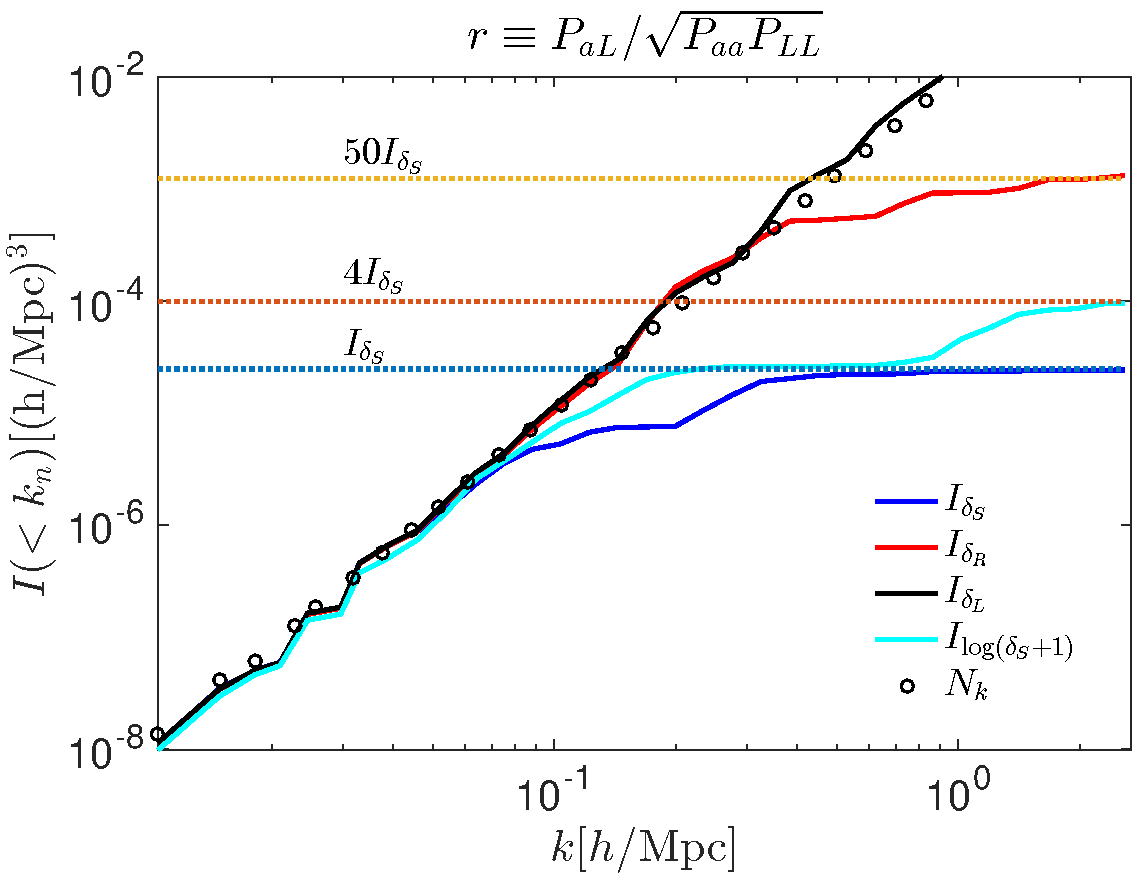
\includegraphics[width=0.48\textwidth]{fig4a.pdf}
    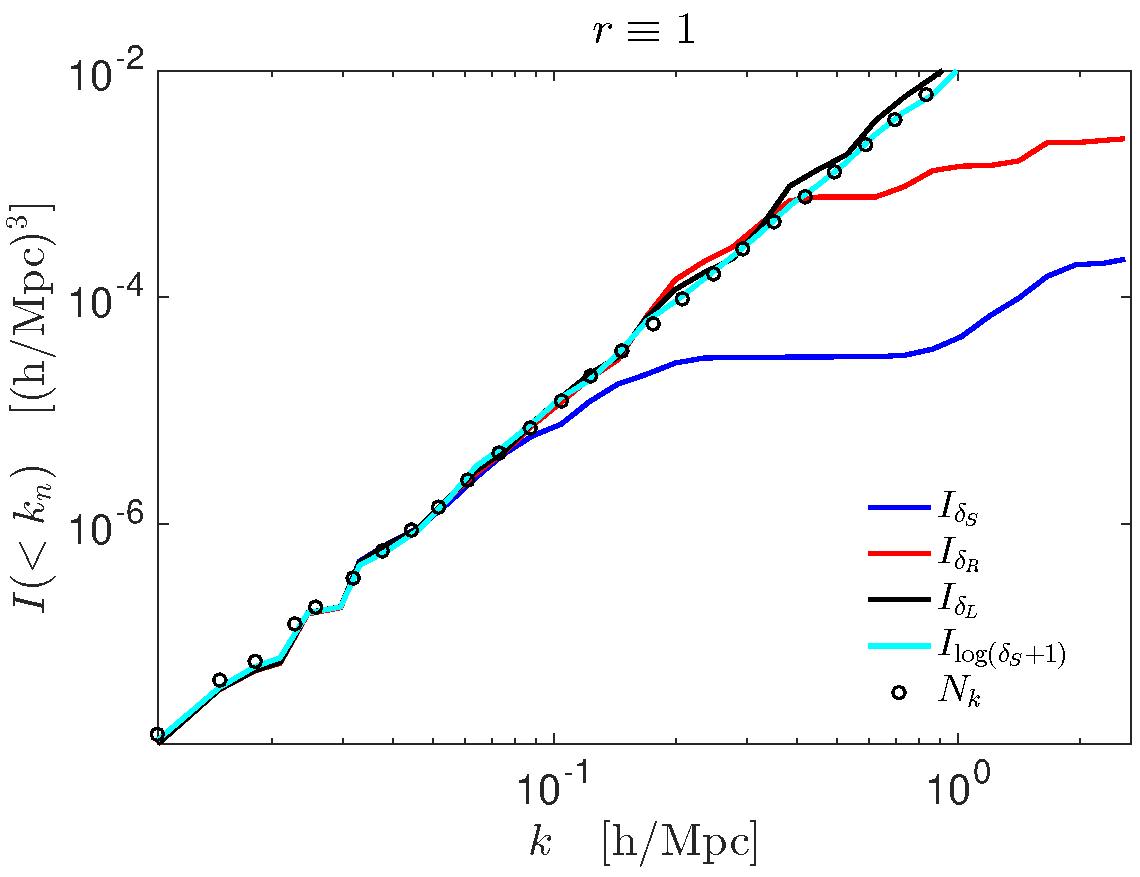
\includegraphics[width=0.48\textwidth]{fig4b.pdf}
    \centering
    \caption{{\it Left.} The Fisher information (solid lines) per unit volume as
      a function of scale.  The blue, red, black curves correspond the power spectra
      of $\delta_S$, $\delta_R$ and $\delta_L$ respectively,
      and the cyan curve
      corresponds to the logarithmic density mapping. The circles
      are the cumulative number of $k$ modes.  Dotted horizontal lines indicate the value of the 
      Fisher information at $k \simeq 2.7$ h/Mpc.  {\it Right.} Same
      as the left panel except with $r\equiv 1$. The black, blue and cyan lines
      match the results in \cite{bib:Rimes2006,bib:Mark2009}.}
  \label{fig:fisherinfo}
\end{figure*}
\end{section}
